\ExTitle{1}
\begin{aufgabe}
\end{aufgabe}
\begin{enumerate}[a)]
	\item Die \underline{Regression} sagt einen reellen Zahlenwert voraus, wogegen die \underline{Klassifikation} eine Klasse vorhersagt.
	\item Regression, da es um die Vorhersage von absoluten Zahlenwerten geht.
	\item Klassifikation, da es um die Vorhersage von Geschlechterklassen geht.
	\item Supervised Learning setzt ein Labeling der Beispieldaten voraus, aus denen der Algorithmus lernen kann. \\
	Bei Unsupervised Learning sind die Beispieldaten nicht gelabelt und der Algorithmus versucht die Daten durch Clustern in verschiedene Klassen zu unterteilen.
	\item
	\begin{enumerate}[i)]
		\item Eine diskrete Zufallsvariable hat eine diskrete Anzhal an Werten, die sie annehmen kann.\\
		Eine kontinuierliche Zufallsvariable kann unendlich viele Werte (of aber nur in einem beschränkten Bereich) annehmen.\\
		Ein Ereignis ist das Ergebnis eines Zufallsexperiments.
		\item Beides sind Funktionen, die die Wahrscheinlichkeit eines Ereignisses (diskret) oder eines x-Achsen Abschnittes (kontinuierlich) abbilden. \\
		Die Wahrscheinlichkeit P(x$\in$A) (A entweder diskreter Wert oder kontinuierliches Intervall) lässt sich dann mithilfe der Funktion/Dichte bestimmen.
		\item Der Erwartungswert einer Zufallsvariablen beschreibt die Zahl, die Zufallsvariable im Mittel annimmt.\\
		Mathematisch: mit x$_i$ Wert und p$_i$ die zugehörige Wahrscheinlichkeit, f(x) ist die Wahrscheinlichkeitsdichte\\
		Diskret: E(X)= $\sum_{i\in I}^{} x_ip_i$\\
		Kontinuierlich: E(X)=$\int^{\infty}_{-\infty}x*f(x) dx$\\
		\item Die \underline{Varianz} Var$(X)$ beschreibt die erwartete quadratische Abweichung der Zufallsvariablen von ihrem Erwartungswert.
		\begin{align*}
			Var(X) &= \sum_{x\in A}(x-\mu)^2P([X=x]) ~\text{(diskret)}\\
			&= \int_{-\infty}^{\infty}(x - \mu)^2 f(x) \text{d}x~\text{(stetig)}
		\end{align*}
		Weiter gilt für die Varianz:
		\begin{align*}
			Var(X) = E((X-E(X))^2) = E(X^2) - E(X)^2~\text{mit }Y = (X-E(X))^2
		\end{align*}
		Also ist $Y$ die quadratische Abweichung von $X$ zu ihrem eigenen Erwartungswert.\\
		Die \underline{Standardabweichung} $\sigma$ ist eine reelle Zahl und ist definiert als:
		\begin{align*}
			\sigma_X = \sqrt{Var(X)}
		\end{align*}
		Sie beschreibt die Streuung einer Zufallsvariable $X$.
		\item Die \underline{Covarianz} $Cov(X,Y)$ beschreibt den monotonen Zusammenhang zweier Variablen und ist definiert als:
		\begin{align*}
			Cov(X,Y) = E[(X - E(X)) \cdot (Y - E(Y))]
		\end{align*}
		Es gibt mehrere Ergebnisfälle:\\
		\begin{center}
			\begin{tabular}{|c|c|}
				\hline 
				$Cov(X,Y)$ & desc \\ 
				\hline 
				$>0$ & Es besteht ein monotoner Zusammenhang \\ 
				\hline 
				$=0$ & Es besteht kein monotoner Zusammenhang \\ 
				\hline 
				$<0$ & Es besteht ein gegenläufig monotoner Zusammenhang \\ 
				\hline 
			\end{tabular} 
		\end{center}
	\end{enumerate} 
	\item Für die Dichtefunktion muss gelten:
	\begin{align*}
		&\int_{-\infty}^{\infty} f(x) \text{d}x = 1\\
		\Rightarrow & \int_{-\infty}^{\infty} [f(x) \cdot g(x)] \neq \int_{-\infty}^{\infty} f(x)\text{d}x \cdot \int_{-\infty}^{\infty} g(x)\text{d}x = 1 \cdot 1 = 1
	\end{align*}
	Somit entsteht bei Multiplikation keine neue Dichtefunktion.
\end{enumerate}
\begin{aufgabe}
\end{aufgabe}
\begin{enumerate}[a)]
	\item $ $\\
	\begin{center}
		\fbox{
			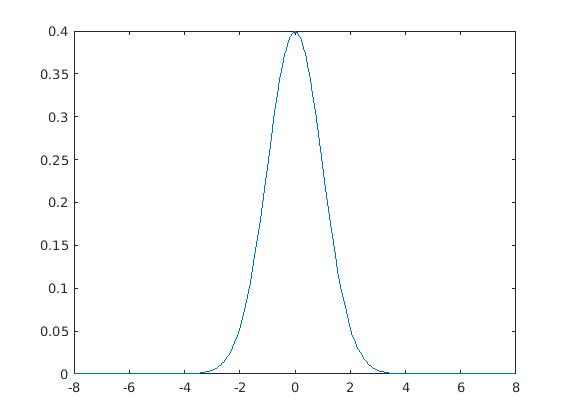
\includegraphics[width=0.4\textwidth]{01/Blatt1_A2a.jpg} %src angabe
		}
	\end{center}\newpage
	\item $ $\\
	\begin{center}
		\fbox{
			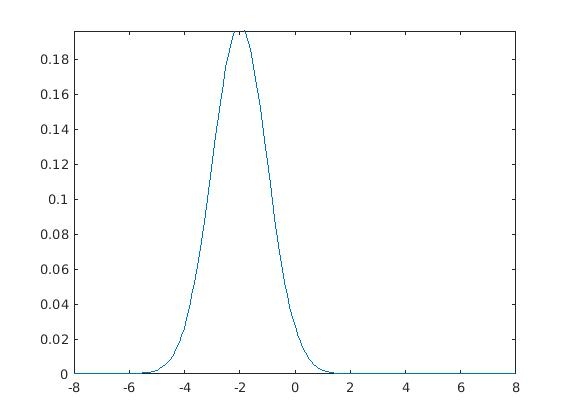
\includegraphics[width=0.4\textwidth]{01/Blatt1_A2b.jpg} %src angabe
		}
	\end{center}
	Der Wert $\mu$ gibt die Verschiebung des Maxima in x-Richtung an, der Graph wird mit -2 also nach links verschoben.\\
	Der Wert $\sigma$ gibt die Stauchung bzw Streckung des Graphen an. Der Graph wird also um den Faktor 2 gestaucht.\\
	\item Um die Wahrscheinlichkeit eines Events innerhalb eines Intervalls zu berechnen wird der Flächeninhalt der Dichtefunktion in diesem Intervall berechnet. \\
	Also: $P(X\in[a,b])=\int^a_bf(x)\text{d}x$
	\item Im Intervall $[\mu\pm\sigma]$ sind 68,27$\%$ aller Werte.\\
	Im Intervall $[\mu\pm2\sigma]$ sind 95,45$\%$ aller Werte.\\
	Im Intervall $[\mu\pm3\sigma]$ sind 99,73$\%$ aller Werte.\\
	\item Die Wahrscheinlichkeitsdichtefunktion kann auch Werte größer als 1 annehmen, solange sie danach normiert ist, solange also das Integral von - Unendlich bis Unendlich gleich 1 ist (per Definition).
\end{enumerate}